	In order to test the coverage of questionnaire features through \gls{cawiml} language and to determine typical frequency of constructs, we have randomly chosen a set of fifteen real questionnaires provided by Pexel. Particularly, we have studied the frequency distribution of \gls{cawiml} vocabulary over this sample of surveys. Figure \ref{fig:eval:frequencies} shows the total number of occurrences for each construct sorted by decreasing order of frequency. The bar chart separates the content, routing and personalisation features with purple, green and blue colours respectively. A more detailed view for this dataset, presented in Table \ref{tab:eval:frequencies}, represents frequency of questionnaire constructs separated for each survey. %It was encouraging to us that all the questionnaires in the sample were represented using \gls{ssm} and apart from the check feature, every other construct was included in any of the surveys chosen. 

	\begin{figure}[H]
	\centering
	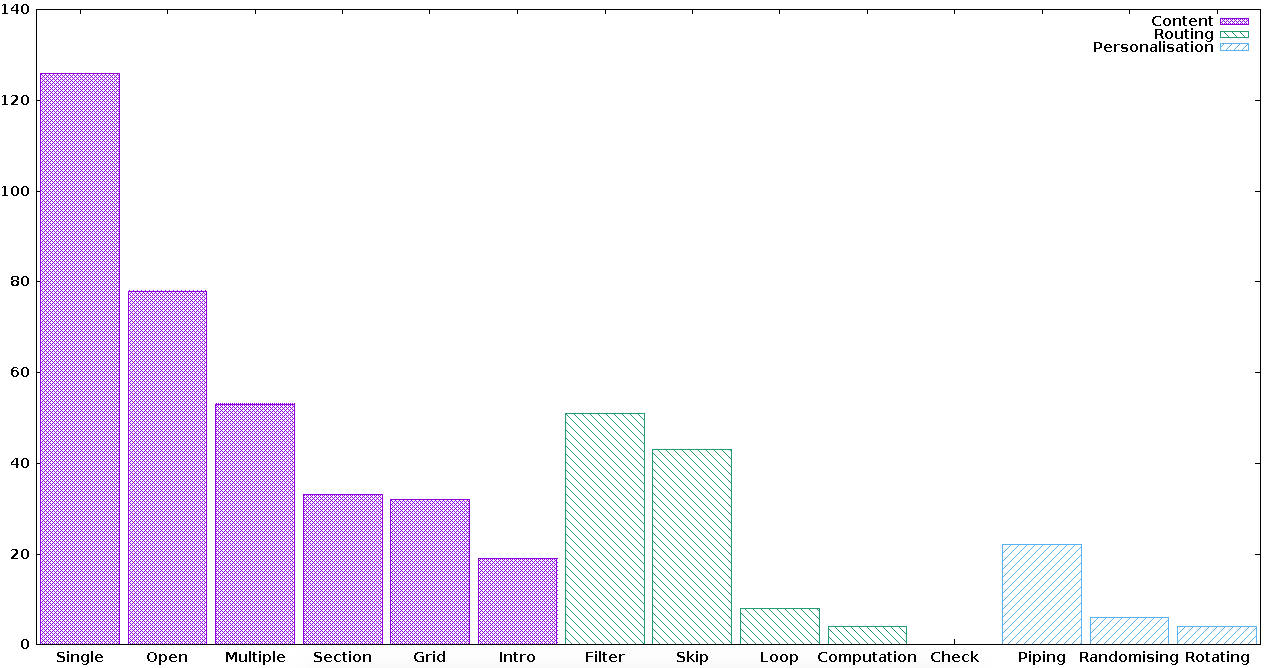
\includegraphics[width=\textwidth]{eval/img/surveyfrequencies.png}
	\caption{Total construct frequencies for fifteen surveys}
	\label{fig:eval:frequencies}
	\end{figure}

	\begin{sidewaystable}
\begin{center}
\begin{tabular}{|c|c|c|c|c|c|c|c|c|c|c|c|c|c|c|c|c|c|}
\hline 
 & Feature & 01 & 02 & 03 & 04 & 05 & 06 & 07 & 08 & 09 & 10 & 11 & 12 & 13 & 14 & 15 & TOTAL\tabularnewline
\hline 
\hline 
\multirow{6}{*}{Content} & Single & 8 & 10 & 7 & 16 & 11 & 8 & 10 & 9 & 2 & 9 & 3 & 9 & 4 & 9 & 11 & 126\tabularnewline
\cline{2-18} 
 & Open-ended & 11 & 1 & 5 & 0 & 11 & 6 & 5 & 1 & 6 & 0 & 12 & 3 & 6 & 9 & 2 & 78\tabularnewline
\cline{2-18} 
 & Multiple & 3 & 0 & 2 & 1 & 1 & 2 & 1 & 6 & 8 & 3 & 8 & 2 & 1 & 7 & 8 & 53\tabularnewline
\cline{2-18} 
 & Section & 1 & 1 & 1 & 7 & 1 & 3 & 2 & 1 & 3 & 5 & 3 & 2 & 1 & 1 & 1 & 33\tabularnewline
\cline{2-18} 
 & Grid & 0 & 0 & 5 & 0 & 1 & 3 & 0 & 1 & 1 & 2 & 0 & 5 & 6 & 7 & 1 & 32\tabularnewline
\cline{2-18} 
 & Intro & 1 & 2 & 1 & 1 & 2 & 1 & 1 & 2 & 1 & 1 & 3 & 0 & 1 & 1 & 1 & 19\tabularnewline
\hline 
\multirow{5}{*}{Routing} & Filter & 1 & 0 & 2 & 0 & 9 & 2 & 0 & 3 & 9 & 3 & 6 & 0 & 5 & 5 & 6 & 51\tabularnewline
\cline{2-18} 
 & Skip logic & 3 & 4 & 1 & 4 & 1 & 5 & 4 & 2 & 2 & 4 & 2 & 4 & 1 & 1 & 5 & 43\tabularnewline
\cline{2-18} 
 & Loop & 0 & 0 & 0 & 0 & 0 & 0 & 0 & 0 & 2 & 0 & 6 & 0 & 0 & 0 & 0 & 8\tabularnewline
\cline{2-18} 
 & Computation & 0 & 0 & 0 & 0 & 0 & 0 & 0 & 0 & 0 & 0 & 0 & 0 & 4 & 0 & 0 & 4\tabularnewline
\cline{2-18} 
 & Check & 0 & 0 & 0 & 0 & 0 & 0 & 0 & 0 & 0 & 0 & 0 & 0 & 0 & 0 & 0 & 0\tabularnewline
\hline 
\multirow{3}{*}{Personalisation} & Piping & 0 & 0 & 3 & 0 & 0 & 0 & 0 & 4 & 9 & 0 & 0 & 0 & 1 & 0 & 5 & 22\tabularnewline
\cline{2-18} 
 & Randomising & 0 & 0 & 0 & 0 & 0 & 0 & 0 & 2 & 1 & 0 & 0 & 0 & 0 & 0 & 3 & 6\tabularnewline
\cline{2-18} 
 & Rotating & 0 & 0 & 0 & 0 & 0 & 0 & 0 & 2 & 0 & 0 & 0 & 0 & 0 & 0 & 2 & 4\tabularnewline
\hline 
\end{tabular}
\caption{Frequency of questionnaire constructs separated by survey}
\label{tab:eval:frequencies}
\end{center}
\end{sidewaystable}


	Firstly, we can confirm that all constructs in our sample of questionnaires were encodable by \gls{cawiml}. Next, in terms of frequency of content, we can observe that single-response questions are most frequent whereas intro constructs were least frequent. Intro question whose purpose is introducing a part of a questionnaire, does not appears once at the beginning instead with each of the sections in the sampled surveys (e.g. questionnaire 04 and 10 with seven and five sections respectively, have only one intro for the entire survey).

	Secondly, for the routing classification, filter construct has obtained the highest number of occurrences, however it does not appear in every questionnaire (e.g. 02, 04, 07, 12). In contrast, the skip feature, although slightly less frequent than filter, is popular amongst the surveys. Therefore, we conclude that skip logic remains an important feature of questionnaires and so should ideally be facilitated by the underlying language of surveys. Computation constructs, become essential when data from one section is needed for another section, but has only been found four times in the questionnaire 13. The absence of check constructs is not surprising since it is a rare feature that tends to appear in less well-designed questionnaires.

	Thirdly, for the personalisation grouping, the three features are presented in the sample tested and piping appears to be the most common construct, specially for populating responses automatically through carry-forward mode. Regarding randomising and rotating constructs, they are less frequent.